\documentclass[a4paper,11pt]{jsarticle}


% 数式
\usepackage{amsmath,amsfonts}
\usepackage{amssymb}
\usepackage{bm}
% 画像
\usepackage[dvipdfmx]{graphicx}
\usepackage{listings,jvlisting}
\lstset{
  basicstyle={\ttfamily},
  identifierstyle={\small},
  commentstyle={\smallitshape},
  keywordstyle={\small\bfseries},
  ndkeywordstyle={\small},
  stringstyle={\small\ttfamily},
  frame={tb},
  breaklines=true,
  columns=[l]{fullflexible},
  numbers=left,
  xrightmargin=0zw,
  xleftmargin=3zw,
  numberstyle={\scriptsize},
  stepnumber=1,
  numbersep=1zw,
  lineskip=-0.5ex
}

\begin{document}

\title{画像実験課題A, B}
\author{1029323422 天野岳洋}
\date{\today}
\maketitle
\clearpage

\section{概要}
ここでは発展課題Aについて取り組んだ内容について述べたのちに, コンテストに対して
取り組んだ内容を述べる. 以後明記はしないが, 伝播層では(B, ?, 1)という形で伝播
するものとし, 逆伝播層では畳み込み層, プーリング層を除き(?, B)という形でデータを
扱っていることに注意したい.
\section{AdvancedA}
発展課題Aの実装について述べる. 実装が簡単であったり,
定義通りにしか実装していない場合は説明は省略もしくは非常に簡単に述べるものとする.
\subsection{A1}
活性化関数としてSigmoid関数の代わりにRELU関数を用いるという内容である.
RELU関数は次のように表せる関数である.
\begin{equation}
  RELU(x)=
  \begin{cases}
    x & \text{if $x \geqq 0$} \\
    0 & \text{if $x < 0$}
  \end{cases}
\end{equation}
また逆伝播は以下のようである
\begin{equation}
  RELU'(x) =
  \begin{cases}
    1 & \text{if $x \geqq 0$} \\
    0 & \text{if $x < 0$}
  \end{cases}
\end{equation}
自分の実装を示す.
\begin{lstlisting}[caption=RELU]
  def __init__(self):
    pass

  def prop(self, x):
    self.input = x
    self.B, self.M, _ = x.shape
    return np.where(x <= 0, 0, x)
    
  def back(self, delta):
    return delta * (np.where(self.input <= 0, 0, 1).reshape(self.B, self.M).T)
\end{lstlisting}

\subsection{A2}
Dropout層を実装せよという内容である. Dropout層の定義は以下のものである.
\begin{equation}
  Dropout(x) =
  \begin{cases}
    x & \text{(ノードが無視されない場合)} \\
    0 & \text{(ノードが無視される場合)}
  \end{cases}
\end{equation}
また逆伝播では,
\begin{equation}
  \begin{split}
    \frac{En}{x} = & \frac{En}{y}\frac{y}{x}  \\= &
    \begin{cases}
      \frac{En}{y} & \text{(ノードが無視されない場合)} \\
      0            & \text{(ノードが無視された場合)}
    \end{cases}
  \end{split}
\end{equation}
具体的な実装の説明に移る.Dropout層のハイパーパラメータを$\rho$とする.
このハイパーパラメータをもとにマスクされるノードの個数を定める.
その後random.choiceによってどのノードがマスクされるかを選択し,
適切な処理をすればよい. またテストの際には定義にのっとり,
マスクはせずに定数倍を行っている.
\begin{lstlisting}[caption=Dropout]
  def __init__(self, phi, M):
    self.phi = phi
    self.msk_num = int(M*phi)
    self.M = M

  def prop(self, x):
    B = x.shape[0]
    M = self.M
    drop_random = np.repeat(np.random.choice(M, self.msk_num), B).reshape(-1, B).T
    mask_vector = np.ones((B, M))
    mask_vector[np.repeat(np.arange(B), self.msk_num), drop_random.flatten()] = 0
    self.msk = mask_vector.reshape(B, -1, 1)
    return x * self.msk

  def back(self, delta):
    return delta * self.msk.reshape(self.B, self.M).transpose(1, 0)

  def test(self, x):
    return x * (1 - self.phi)
\end{lstlisting}
prop層のmask\_vectorの作り方が少し複雑なので, 例を挙げて説明する.
例えば, msk\_num = 3, M = 5, B = 2の時を考える. 今drop\_randomは
0$\sim$4から3個重複を許さずに選び, それを2回ずつ繰り返し, 次元を(3, 2)に変え転置をとるものだから, 順番に追っていくと,
例えば, 0, 1, 3が選ばれたとすると, 次のような形で処理が行われ, drop\_randomが得られることとなる.

$$
  [0, 1, 3] \rightarrow [0, 0, 1, 1, 3, 3] \rightarrow
  \begin{bmatrix}
    0 & 0 \\
    1 & 1 \\
    3 & 3 \\
  \end{bmatrix}
  \rightarrow \begin{bmatrix}
    0 & 1 & 3 \\
    0 & 1 & 3 \\
  \end{bmatrix}
$$
続いて同様にmask\_vectorの推移を説明する. まず, (B, M)の形で全て1
が入ったもので初期化され, その後mask\_vector[[0,0,0,1,1,1][0 1 3 0 1 3]] = 0
となっている. つまり

$$
  mask\_vector \rightarrow \begin{bmatrix}
    1 & 1 & 1 & 1 & 1 \\
    1 & 1 & 1 & 1 & 1
  \end{bmatrix} \rightarrow
  \begin{bmatrix}
    0 & 0 & 1 & 0 & 1 \\
    0 & 0 & 1 & 0 & 1
  \end{bmatrix}
$$
というような推移になっている. あとはこれを適切な形に変形させ,
入力データとアダマール積をとればあるノードの出力が0になっていることが
簡単にわかる. また逆伝播層でも入力のshapeが違うことを除けば同様に
アダマール積をとるだけである.
\subsection{A3}
Batch-Normalizationを行えというものである.
定義式は教科書のとおりである. 実装は定義通り行った.
ここでは実際の実装を添付するのみとする.
\begin{lstlisting}[caption=Batch-Normalization-prop]
  def prop(self, x):
    #x = B * M * 1
    self.x = x
    self.B, self.M, _ = x.shape
    self.microB = np.sum(x, axis=0) / x.shape[0]
    self.sigmaB = np.sum((x - self.microB) ** 2, axis=0) / x.shape[0]
    self.normalize_x = (x - self.microB) / np.sqrt(self.sigmaB + BatchNormalize.eps)
    self.y = self.ganma * self.normalize_x + self.beta
    # yをreturn
    return self.y
\end{lstlisting}

\begin{lstlisting}[caption=Batch-Normalization-back]
  def back(self, delta):
    delta_xi_head = delta * self.ganma
    delta_sigmaB2 = np.sum(delta_xi_head * (self.x.reshape(self.B, self.M).T - self.microB) * (-1/2) * np.power(self.sigmaB + BatchNormalize.eps, -3/2), axis=1).reshape(self.M, 1)
    delta_microB = np.sum(delta_xi_head * (-1 / np.power(self.sigmaB + BatchNormalize.eps, 1/2)), axis=1).reshape(self.M, 1) + (-2) * delta_sigmaB2 * np.sum(self.x.reshape(self.B, self.M).T - self.microB, axis=1).reshape(self.M, 1)
    delta_a = delta_xi_head * np.power(self.sigmaB + BatchNormalize.eps, -1/2) + delta_sigmaB2 * 2 * (self.x.reshape(self.B, self.M).T - self.microB) / self.B + delta_microB / self.B
    delta_ganma = np.sum(delta * self.normalize_x.reshape(self.B, self.M).T, axis=1).reshape(self.M, 1)
    delta_beta = np.sum(delta, axis=1).reshape(self.M, 1)
\end{lstlisting}

\subsection{A4}
様々な最適化手法を試すものとなっている. 実際の実装は以下のようである.
\begin{lstlisting}
  def adagrad(self, w_b, delta, h):
    h = h + delta * delta
    return w_b - Batch.my * np.power(h, -1/2) * delta, h

  def RMSProp(self, w_b, delta, h):
    h = Batch.rho * h + (1 - Batch.rho) * delta * delta
    return w_b - Batch.my * (1 / (np.power(h, 1/2) + Batch.eps) ) * delta, h

  def AdaDelta(self, w_b, delta, h, s):
    h = Batch.rho * h + (1 - Batch.rho) * delta * delta
    delta_w = - np.power(s + Batch.eps, 1/2) * np.power(h + Batch.eps, -1/2) * delta
    s = Batch.rho * s + (1 - Batch.rho) * delta * delta
    w = w_b + delta_w
    return w, h, s

  def Adam(self, w_b, delta, t, m, v):
    t = t + 1
    m = Batch.beta1 * m  + ( 1 - Batch.beta1 ) * delta
    v = Batch.beta2 * v  + ( 1 - Batch.beta2 ) * delta * delta
    m_head = m / ( 1 - np.power(Batch.beta1, t))
    v_head = v / ( 1 - np.power(Batch.beta2, t))
    W = w_b - Batch.alpha_para * m_head / (np.power(v_head, 1/2) + Batch.eps)
    return W, m, v, t
\end{lstlisting}
実装の方法は省略するものとし, それぞれの学習方法がどのようなものであるかを考察する.

\subsubsection*{Momentum付きSGD}
SGDでは振動してしまい収束しないという状況が考えられる.
Momentum付きSGDでは現在の勾配だけでなく, 過去の差分を用いることによって,
この振動を抑えている.

例えば$ y = x^2 $のグラフにおいて今の地点が$x = 1$であり, 学習率が1であった場合, 
次の地点は$x = -1$となりさらにその次は$x = 1$となり振動してしまう.
一方で, Momentum付きSGDにすることによって, 解消される. 例えば, 0.9だけ過去の差分を取り入れるとしたら, 
$x = 1$の次は, $x = - 1$でありさらにその次は, $\Delta = 0.9 * -2 + 1 * 2 = 0.2$であるので, $x = -1 + 0.2 = -0.8$...となり
振動が抑えられていることがわかる.
\subsubsection*{AdaGrad}
学習率を調節するものである. SGDの問題として, 収束速度が各軸によってまばらで
あるという問題がある. 具体的に言うと, ある軸で見たときに勾配が緩やかな状況を考えると, 
その軸での更新幅は小さく, それ以外の軸での更新幅は大きいということが起こる. すなわち, 学習を進めた際に
それ以外の軸では収束しているのに, その軸が収束していないという状況が考えられる.
これを解消するために, 更新が少ない軸では更新幅を大きくするという学習率の面での工夫がAdaGradである.
教科書のhは今までの更新の2乗の総和であり, hが大きい場所程更新幅は小さい。またその逆もしかりである.
\subsubsection*{RMSProp}
AdaGradでは一度大きな更新が行われた軸では学習率が大きく下がってしまったままという問題が発生した.
その問題を解決するために, hを今までの単なる総和ではなく, 等比数列的に過去の更新幅を減衰していって加えていくという
変更を加えたものである. またこのような処理を加えることによって, hが0に収束してしまう場合が考えられるので, 
0割りを防ぐために$\epsilon$が分母に加えられている.
\subsubsection*{Adadelta}
RMSProp以下では, $\Delta w$の次元が$w$とマッチしていないという事態になっていた.
実際, $\Delta w$は基本的に勾配の定数倍であったので, その次元はwの次元を$Dimw$とすると, 
$1/Dimw$となる. 
これは微分が損失関数の変位(定数)をwで割ったものの微小極限であることを考えれば明らかである.
よって$w + \Delta w$は次元が違う二つの値を足していることとなる.
そのため, なにか不都合な問題が起こった(何が問題なのかを調べきることができませんでした.)
これを解決するのがAdadeltaである. 実際に次元を見てみると, 
hの次元は $1 / Dimw^2$であり, $s$の次元を$Dimw^2$とすると, $\Delta w$の次元は
$Dimw * Dimw / Dimw = Dimw$となり, うまくいっている.\footnote{$s$の次元を知るのに, $\Delta w$の次元が必要で, 
その逆も成り立つので, 一度仮定が必要になっています. うまく示せていませんね...}
\subsubsection*{Adam}
Momentum + RMSPropである. これは式を見えれば簡単に理解できる.
(54), (55)の補正について説明する.
(54)の説明だけで十分である. 簡易的に一次元値であることを仮定し, さらに$\beta_1$
を$\beta $としている. 教科書式(52)を変形していく.
$\frac{\delta E_n}{\delta W}$ をgとする.
\begin{align*}
  m_t = & (1 - \beta)g_t + \beta m_{t-1}  \\
      = & (1 - \beta)g_t + \beta (1 - \beta)(g_{t-1}) + \beta^2 m_{t-2} \\
      = & \dots \\
      = & (1 - \beta)\sum_{i=1}^{t}\beta^{t-i}g_i + \beta^{t}m_{0}
\end{align*}
ここで$g_t$と$m_t$の平均についての関係性を調べると
\begin{align*}
  \mathbb{E}\lbrack m_t \rbrack = & \mathbb{E}\lbrack (1 - \beta)\sum_{i=1}^{t}\beta^{t-i}g_i + \beta^{t}m_{0} \rbrack \\
  = & (1-\beta)\sum_{i=1}^{t}\beta^{t-i}\mathbb{E}\lbrack g_i \rbrack + \beta^t\mathbb{E}\lbrack m_0 \rbrack \\
  = & (1 - \beta)\mathbb{E}[g_t]\frac{1-\beta^t}{1-\beta} \\
  = & (1 - \beta^t)\mathbb{E}[g_t]
\end{align*}
よって不偏性を保つために, 式(54)によって補正していることが分かった.\footnote{そもそもなぜ不偏性が必要なのかがわからなかった.時間とともに, mtの値が大きくなっていくのが問題?}
\subsection{A5}
まだできてません.
\subsection{A6}
畳み込み層の実装を行う.
以下の手順で畳み込み層の実装を行った.
\begin{enumerate}
  \item 畳み込みフィルタを定義する。初期化は今回正規分布に従う値にした.
  \item 入力データを畳み込みフィルタを適用するために、フィルタサイズに合わせて切り分ける。
  \item それぞれの切り分けられた部分に対して畳み込みフィルタを適用し、その結果を適切に並べたものを出力とする。
  \item バイアスを加える.
\end{enumerate}
特に, 2.が非常にややこしいのでこの部分を説明する. 
\subsubsection{切り分け}
切り分けであるが, 今回は畳み込み前後でサイズが変わらないほうが嬉しいため, 
フィルタサイズは奇数長であるという制限を設けている.さらにこの切り分けの前に, paddingを行っている.
paddingはnumpy.padで簡単に実装できる.
まずは切り分けを行うコードを提示する.
\begin{lstlisting}[caption=x2X]
  def x2X(self, x, R):
    B, ch, x_length, x_width = x.shape
    dx = x_length - R + 1
    dy = x_width - R + 1
    altx = np.zeros((B, ch, R, R, dx, dy))
    for i in range(R):
        for j in range(R):
            altx[:, :, i, j, :, :] = x[:, :, i:i+dx, j:j+dy]
    return altx.transpose(1, 2, 3, 0, 4, 5).reshape(R*R*ch, dx*dy*B)
\end{lstlisting}
順に説明を行う. xは切り分けを行う前のテンソルであり, Rはフィルタサイズになっている.
ここでまず, xのシェイプから各種値を取得している. 次から具体的な切り分けの作業を行っていくが, 
まずfor文を使う回数をなるべく少なくするために, 大きな四角形でくりぬくことで, 切り分け後の一行一列目の値だけを並べたものを
取得できる. このようにすることで繰り返し数をフィルタサイズ * フィルタサイズ程度に収めることができる.
図を使って説明を行う. 以下の図はB = 1, ch = 1 であることに注意したい.
\begin{figure}[h]
  \centering
  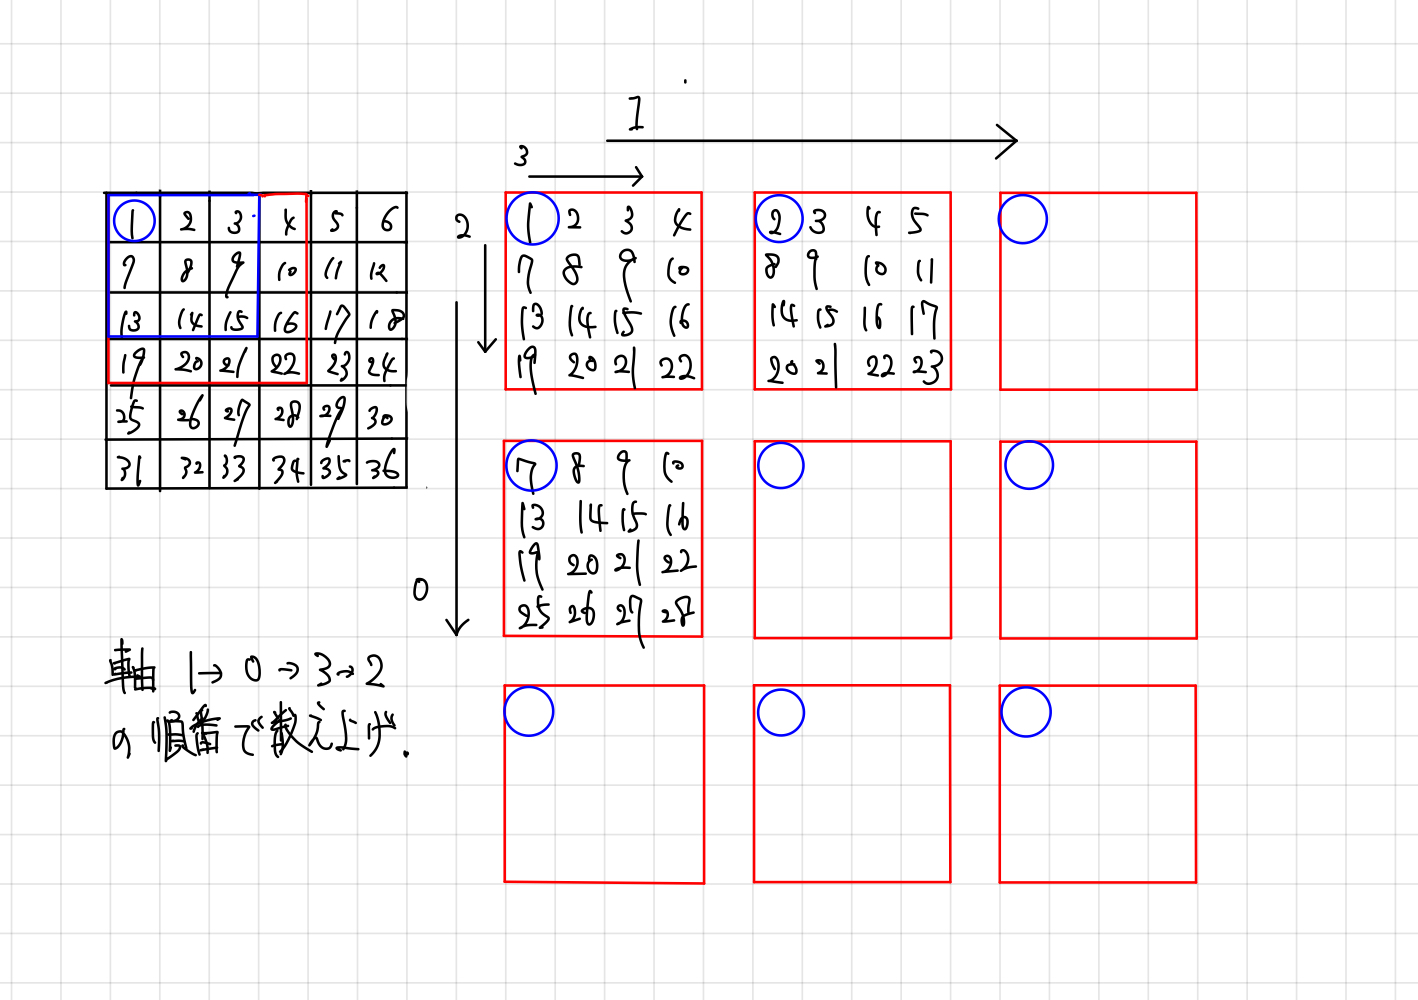
\includegraphics[height = 7cm]{rep_conv.jpg}
  \caption{x2X}
\end{figure}
赤四角の大きさがdx, dyである. 左の大きなテンソルの初期化を次に行っている.
その次のfor文内でそのテンソルにくりぬいている.
最後のtransposeが数え上げの順番を変えている.その後にreshapeで適切な形にしている.

\subsubsection*{適用}
切り分けさえできれば後はたやすい. 順伝播は次のようなものになる.
\begin{lstlisting}[caption=convlution-prop]
  self.B = x.shape[0]
    r = self.R // 2
    self.r = r
    x_prime = np.pad(x, [(0,), (0, ), (r,), (r,)], "constant")
    self.X = self.x2X(x_prime, self.R)
    self.Y = np.dot(self.filter_W, self.X) + self.bias
    # self.Y -> K * (imgsize * B)
    self.Y = self.Y.reshape(self.K, self.B, self.imr, self.imr).transpose(1, 0, 2, 3)
    # self.Y -> B * K * imlen * imlen
    return self.Y
\end{lstlisting}

\subsubsection*{逆伝播}
教科書通りの実装である.
気をつけなければならない点として, x2Xの逆の作業を行う必要があることと,
paddingを行っているのでその部分を切り取ったものを出力しなければならないことがあるが, 
それ以外は簡単である.
\begin{lstlisting}[caption=X2x]
  def X2x(self, X):
    w = self.R
    bigL = self.imr + self.r*2 - w + 1
    bigW = self.imr + self.r*2 - w + 1
    x = np.zeros((self.B, self.ch, self.imr + self.r * 2, self.imr + self.r * 2))
    arX = X.reshape(self.ch, w, w, self.B, bigL, bigW).transpose(3, 0, 1, 2, 4, 5)
    for i in range(w):
        for j in range(w):
            x[:, :, i:i+bigL, j:j+bigW] = arX[:, :, i, j, :, :]
    return x
\end{lstlisting}
\begin{lstlisting}[caption=convlution-back]
  def back(self, delta):
    #delta -> B * K * imlen * imlen
    delta = delta.transpose(1, 0, 2, 3).reshape(self.K, -1)
    #delta -> K * (B * imlen * imlen)
    delta_filter_x = np.matmul(self.filter_W.T, delta)
    delta_filter_W = np.matmul(delta, self.X.T)
    delta_filter_b = np.sum(delta, axis=0)
    self.filter_W = self.filAdam.update(delta_filter_W)
    self.bias = self.biAdam.update(delta_filter_b)
    return self.X2x(delta_filter_x)[:, :, self.r:self.r + self.imr, self.r:self.r + self.imr]
\end{lstlisting}


\subsection{A7}
プーリングを行う.今回はMaxPoolingを行うものとする.
以下の手順での実装とする.
\begin{enumerate}
  \item 切り分けを行い, その窓ごとの最大値とその位置を取得
  \item 適切な形に変形
  \item 取得した位置をもとに, 逆伝播してきた微分値を代入.
  \item x2Xの逆の作業によって適切な形に変形
\end{enumerate}

全て以前に出てきたものであるので実装は簡単であるが, 
想像がつきづらいので, B = 1, ch = 1, の状況下で具体的に説明を行う.
まずは以下の図を見てもらいたい.

\begin{figure}[h]
  \centering
  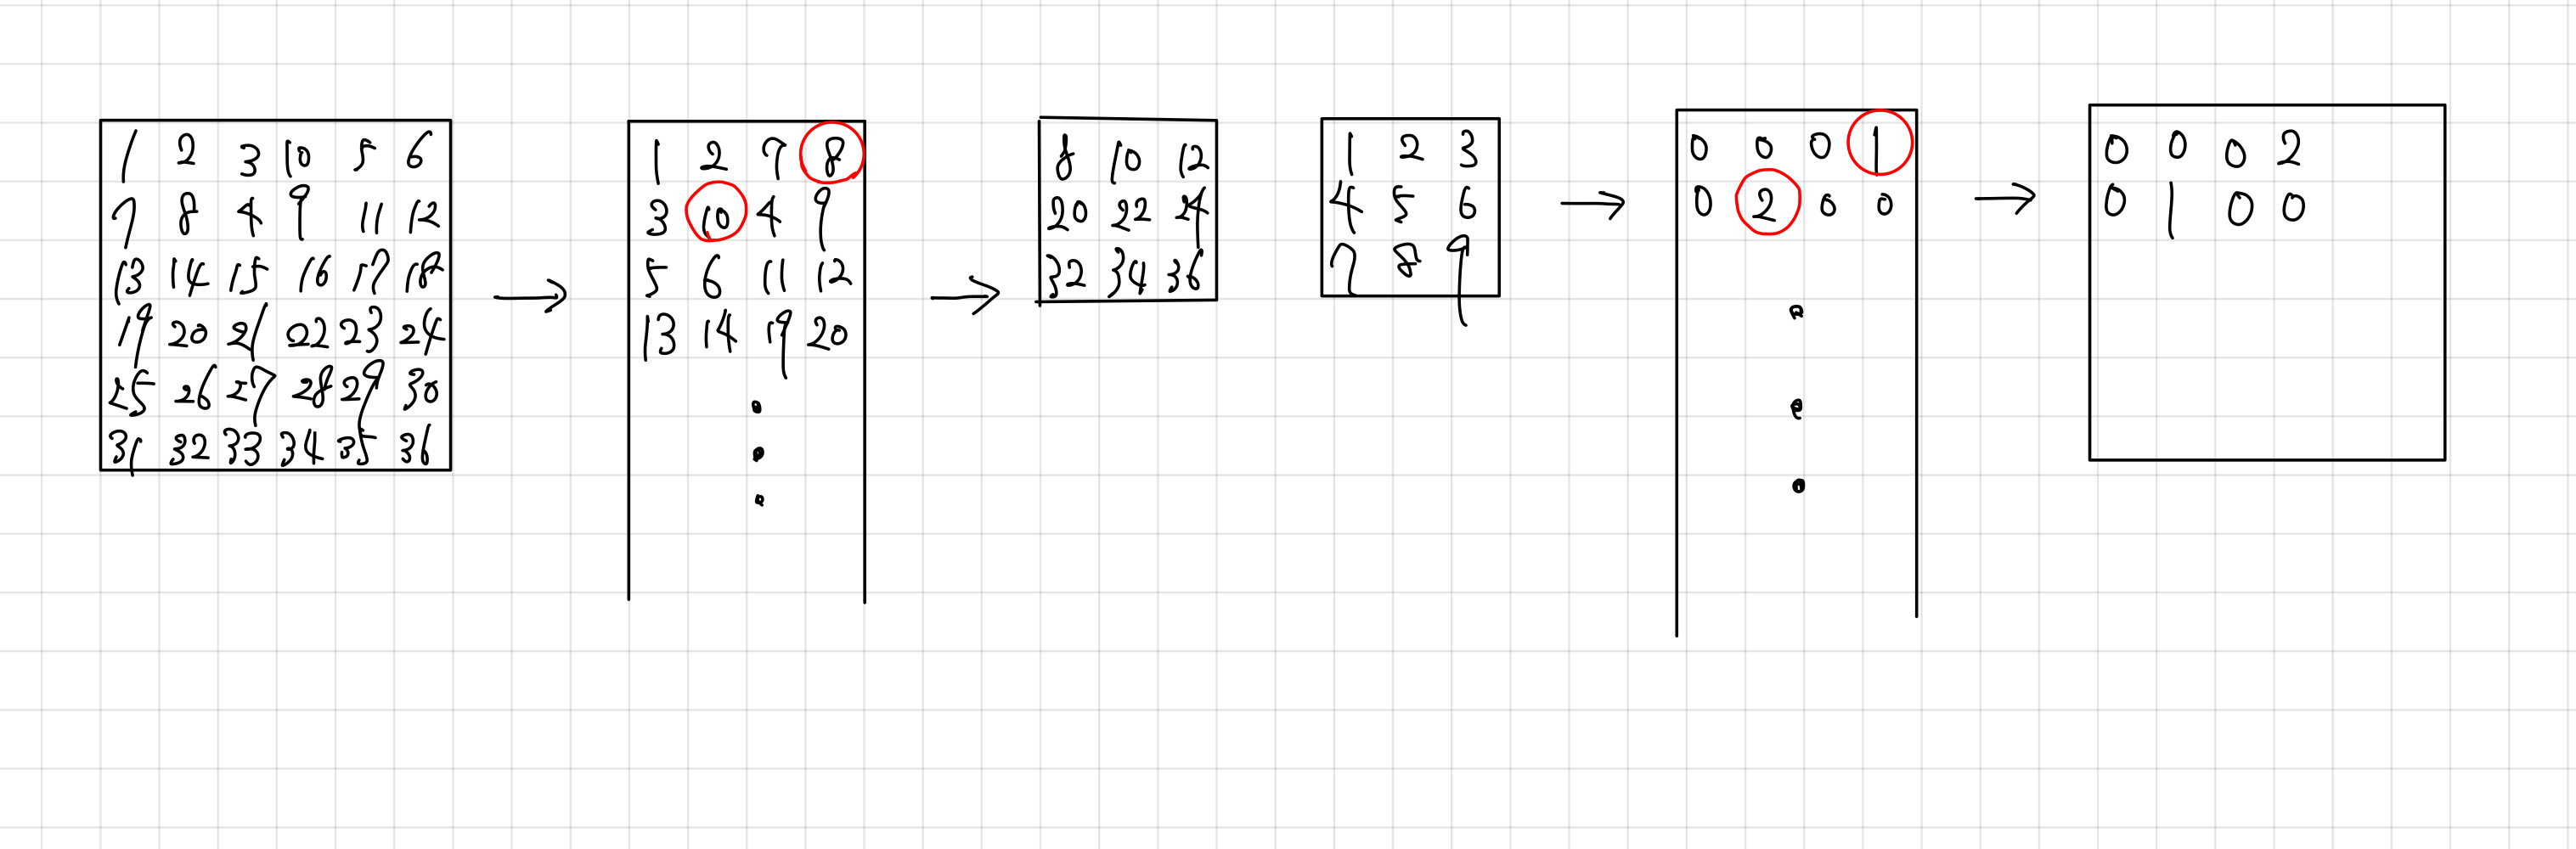
\includegraphics[height = 5cm]{pooling.jpg}
  \caption{pooling}
\end{figure}
まずストライドつきのx2Xを行っている.その後argmaxによって, 最大値を取得する位置を取得している.
これは逆伝播の際に必要になる. そして最大値を取得して, 適切な形に変形すれば, 順伝播は終了である.
次に逆伝播であるが, これはdeltaの形が小さくなったもので得られることに注意し, 0で初期化したものに, 
最大値の位置にdeltaを平坦にしたものを代入すればよい. そしてストライド付きのX2xで適切な形に変形すればよい.

実際の実装は以下のとおりである.
\begin{lstlisting}[caption=pooling\_x2X]
  def x2X(self, x):
    w = self.w
    bigL = self.iml - w + 1
    bigW = self.imw - w + 1
    arrayX = np.zeros((self.B, self.ch, w, w, self.outl, self.outw))
    for i in range(w):
        for j in range(w):
            arrayX[:, :, i, j, :, :] = x[:, :, i:i+bigL:w, j:j+bigW:w]
    X = arrayX.transpose(0, 1, 4, 5, 2, 3).reshape(-1, w*w)
    return X
\end{lstlisting}
ストライドが追加されていることに注意したい. ストライド幅はプーリングサイズに等しい.

\begin{lstlisting}[caption=pooling\_prop]
  def pooling(self, x, w):
    self.w = w
    self.B, self.ch, self.iml, self.imw = x.shape
    self.outl = self.iml // w
    self.outw = self.imw // w
    X = self.x2X(x)
    self.arg_max = np.argmax(X, axis = 1)
    output1 = np.max(X, axis=1).reshape(
        self.B, self.ch, self.outl, self.outw)
    output2 = output1.transpose(1, 0, 2, 3).reshape(self.B, -1, 1)
    return output1
\end{lstlisting}

\begin{lstlisting}[caption=pooling\_X2x]
  def X2x(self, X):
    w = self.w
    bigL = self.iml - w + 1
    bigW = self.imw - w + 1
    x = np.zeros((self.B, self.ch, self.iml, self.imw))
    arX = X.reshape(self.B, self.ch, self.outl, self.outw, w, w).transpose(0, 1, 4, 5, 2, 3)
    for i in range(w):
        for j in range(w):
            x[:, :, i:i+bigL:w, j:j+bigW:w] = arX[:, :, i, j, :, :]
    return x
\end{lstlisting}

\begin{lstlisting}[caption=pooling\_back]
  def back(self, delta):
    #delta ->  B * (ch* imglen) 
    w = self.w
    delta_x = np.zeros((delta.size, w * w))
    delta_x[np.arange(self.arg_max.size), self.arg_max.flatten()] = delta.flatten()
    return self.X2x(delta_x)
\end{lstlisting}

\section{contest}
コンテストに挑戦した過程を大まかに述べる
以下は最終的な構成である.
\subsection{Data-argumentation}
\subsubsection{Affine変換}
\subsubsection{gause-noise}
\subsubsection{thickfiltering}
\subsection{Convlution}
\subsection{pooling}
\subsection{}
\subsection{}
\section*{不採用群}
\subsubsection{optimaizer:SAM}
\subsubsection{pseudo-labeling1}
\subsubsection{randomcrop}
\subsubsection{randomerasing}
\subsubsection{mixup}
\subsubsection{cutout}
\subsubsection{label-smoothing}

\section{B}
自宅デスクトップでの環境構築からGAN作成までの手続きを述べる.
\subsection{環境}

\subsection{環境構築}

\subsection{環境構築check}
\begin{lstlisting}[caption=check]
  from tensorflow.python.client import device_lib

    print(device_lib.list_local_devices()) 
  
\end{lstlisting}


\end{document}